\chapter{Технологическая часть}

% =====================================================
\section{Формат входных и выходных данных}

Входные данные располагаются в текстовом файле определённого формата.

Каждый тип объектов представляется в файле следующим образом:

\begin{itemize}

\item Сфера:

\begin{enumerate}[label=\arabic*)]
    \item тип объекта (s) и название;
    \item координаты центра (три вещественных числа, задающих координаты соответственно по $x$, $y$ и $z$);
    \item радиус (вещественное положительное число);
    \item оптические параметры вещества.
\end{enumerate}

\item Пузырь:

\begin{enumerate}[label=\arabic*)]
    \item тип объекта (b) и название;
    \item описание внешней сферы;
    \item описание внутренней сферы.
\end{enumerate}

\item Триангулированный объект:

\begin{enumerate}[label=\arabic*)]
    \item тип объекта (t) и название;
    \item координаты вершины (три вещественных числа, задающих координаты соответственно по $x$, $y$ и $z$), перед которыми v;
    \item поверхность, описанная номерами трёх вершин (целые числа от 0 до N, где N -- количество вершин), перед которыми f;
    \item оптические параметры вещества.
\end{enumerate}

\clearpage

\item Источник света:
\begin{enumerate}[label=\arabic*)]
    \item тип объекта (l);
    \item координаты расположения (три вещественных числа, задающих координаты соответственно по $x$, $y$ и $z$);
    \item интенсивность (вещественное число от 0 до 1).
\end{enumerate}

\end{itemize}

Оптические параметры вещества задаются следующим образом:

\begin{enumerate}[label=\arabic*)]
    \item цвет объекта (три целочисленных переменных в модели RGB);
    \item коэффициенты фоновый, диффузный, зеркальный и пропускания (вещественные числа от 0 до 1);
    \item показатель отражения (вещественное неотрицательное число);
    \item показатель преломления (вещественное неотрицательное число);
    \item дисперсия (вещественное неотрицательное число).
\end{enumerate}

\begin{center}
\captionsetup{justification=raggedright,singlelinecheck=off}
\begin{lstlisting}[label=lst:ray_1,caption=Пример входного файла с триангулированным объектом и источником света,basicstyle=\ttfamily\footnotesize]
t тетраэдр
v 500.0 300.0 0
v 700.0 300.0 -300.0
v 300.0 400.0 0
v 300.0 350 -100.0
f 1 3 4
f 1 2 4
f 2 3 4
f 1 2 3
-
255 255 255
0.3 1 0 0
100
1
0

l
1000 1000 1000
0.5
\end{lstlisting}
\end{center}

\clearpage

\begin{center}
\captionsetup{justification=raggedright,singlelinecheck=off}
\begin{lstlisting}[label=lst:ray_1,caption=Пример входного файла со сферой и пузырём,basicstyle=\ttfamily\footnotesize]
s сфера
300 400 150
100
0 0 255
0.4 0.1 0 1
100
1
0

b пузырь
450 150 -100
100
100 100 100
0.1 0.4 0 1
100
1.3
100000
450 150 -100
99.9
0 0 0
0 0 0.5 1
0
1
0
\end{lstlisting}
\end{center}

На выходе пользователь получает изображение в цветовой модели $RGB$ с разрешением ${960}\times{960}$ и расширением $PNG$.


% =====================================================
\section{Средства реализации}

В качестве языка программирования для реализации программного обеспечения был выбран $C++$ \cite{c++}, так как он позволяет реализовать все алгоритмы, выбранные в результате проектирования и поддерживает все структуры данных.

Был выбран фреймворк $Qt$ \cite{qt} для реализации интерфейса программного обеспечения, так как в нём присутствуют инструменты для работы с изображениями и интерфейсом.

% =====================================================
\section{Описание используемых классов}

При реализации программы использовался объектно-ориентированный подход. Реализованы следующие классы и структуры:

\begin{itemize}
    \item класс MainWindow -- содержит информацию об интерфейсе и связи кнопок с действиями;
    \item класс Loader -- описывает действия загрузки данных из файла и построения соответствующих объектов на основе прочитанной информации;
    \item класс Scene -- описывает сцену (объекты, источники света), методы взаимодействия со сценой и ее объектами;
    \item класс Light -- описывает расположение и интенсивность источника света, а также методы взаимодействия с ним;
    \item класс Object -- описывает представление трёхмерного объекта в программе и методы работы с ним;
    \item класс TriangulatedObject -- описывает трехмерный объект, состоящий из треугольных полигонов и методы работы с ним;
    \item класс Triangle -- описывает полигон для представления трёхмерного объекта и методы работы с ним;
    \item класс Sphere -- описывает сферу и методы работы с ней;
    \item класс Bubble -- описывает пузырь, содержащий две сферы, и методы работы с ним;
    \item класс Substance -- описывает свойства материала объекта;
    \item класс Ray -- описывает трассируемый луч.
\end{itemize}

\clearpage

% =====================================================
\section{Примеры реализации алгоритов}

В листингах \ref{lst:ray_1}-\ref{lst:ray_2} представлена реализация алгоритма трассировки лучей. В листинге \ref{lst:tr} представлена реализация алгоритма поиска пересечения луча с триангулированным объектом. В листинге \ref{lst:s} представлена реализация алгоритма поиска пересечения луча со сферой.

\begin{center}
\captionsetup{justification=raggedright,singlelinecheck=off}
\begin{lstlisting}[label=lst:ray_1,caption=Трассировка лучей (часть 1),basicstyle=\ttfamily\footnotesize]
QColor Scene::TraceRay(Ray ray, double min_dist, double max_dist, int trace_depth, bool where)
{
    QColor color = QColor(0, 0, 0);
    auto [flag, closest, intersection, normal] = findClosestIntersection(ray.start_point, ray.direction, min_dist, max_dist);
    if (flag == NOTHING) return color;
    if (trace_depth == max_trace_depth) return color;
    double reflectK = 0.0;
    QColor reflectColor = QColor(0, 0, 0);

    if (objects[closest]->getSubstance().getCoefficients() .specular > EPS)
    {
        QVector3D reflectDir = getReflectVector(ray.direction, normal).normalized();
        Ray reflectRay = {
            .start_point = intersection,
            .direction = reflectDir,
            .color = ray.color,
            .len = ray.len,
            .n = ray.n,
        };
        reflectColor = TraceRay(reflectRay, min_dist, max_dist, trace_depth + 1, where);
        double rC = getInterferenceColor(ray.color, objects[closest]->getSubstance());
        reflectK = getInterferenceStrengthCoef(objects[closest] ->getThickness(), rC, ray.direction, normal, ray.len);
    }

    QColor refractColor = QColor(0, 0, 0);
\end{lstlisting}
\end{center}

\clearpage

\begin{center}
\captionsetup{justification=raggedright,singlelinecheck=off}
\begin{lstlisting}[label=lst:ray_2,caption=Трассировка лучей (часть 2),basicstyle=\ttfamily\footnotesize]
    if (objects[closest]->getSubstance().getCoefficients(). refract > EPS) 
    {
        double rC = getInterferenceColor(ray.color, objects[closest]->getSubstance());
        QVector3D refractDir = getRefractVector(ray.direction, normal, rC, ray.n, where).normalized();
        Ray refractRay = {
            .start_point = intersection,
            .direction = refractDir,
            .color = ray.color,
            .len = ray.len,
            .n = rC,
        };
        refractColor = TraceRay(refractRay, min_dist, max_dist, trace_depth + 1, !where);
    }

    double intensity = 0.0;
    double specIntensity = 0.0;

    for (int i = 0; i < lights.size(); i++) 
    {
        QVector3D light = intersection - lights[i].getView();
        double k = findLightIntensity(intersection, (-1) * light, MIN_DIST_LIGHT, MAX_DIST_LIGHT);
        if (!k) continue;
        light.normalize();
        intensity += k * lights[i].getIntensity() * std::max(0., scalarProduct(normal, (-1) * light));
        QVector3D reflect = (getReflectVector(light, normal)).normalized();
        specIntensity += pow(std::max(0., scalarProduct(reflect, (-1) * ray.direction)), objects[closest]->getSubstance().getSpecularIndex()) * lights[i].getIntensity() * k;
    }

    QColor diffColor = objects[closest]->getSubstance().getColor();
    color = getColor(intensity, specIntensity, objects[closest]->getSubstance().getCoefficients(), diffColor, reflectColor, refractColor, reflectK, trace_depth);
    return color;
}
\end{lstlisting}
\end{center}

\clearpage

% =====================================================
\begin{center}
\captionsetup{justification=raggedright,singlelinecheck=off}
\begin{lstlisting}[label=lst:tr,caption=Поиск пересечения луча с триангулированным объектом,basicstyle=\ttfamily\footnotesize]
std::tuple<QVector3D, QVector3D, double> TriangulatedObject::getIntersectionInfo(QVector3D start_point, QVector3D direction, double min_dist, double max_dist)
{
    double min_t = max_dist;

    QVector3D closest_point(0, 0, 0);
    QVector3D closest_normal(0, 0, 0);

    auto [intersection, normal, t] = sphere.getIntersectionInfo(start_point, direction, min_dist, max_dist);

    if (t == max_dist)
        return { closest_point, closest_normal.normalized(), min_t };

    for (int i = 0; i < faces.size(); i++)
    {
        Triangle cur_face = faces[i];
        if (scalarProduct(cur_face.getNormal(), direction) >= 0) continue;
        if (!cur_face.isIntersection(direction)) continue;
        auto [point, t] = cur_face.findIntersection(start_point, direction);
        if (!cur_face.isInside(point)) continue;

        if (t < min_t && t > min_dist && t < max_dist)
        {
            min_t = t;
            closest_point = point;
            closest_normal = cur_face.getNormal();
        }
    }

    return { closest_point, closest_normal.normalized(), min_t };
}
\end{lstlisting}
\end{center}

\clearpage

% =====================================================

\begin{center}
\captionsetup{justification=raggedright,singlelinecheck=off}
\begin{lstlisting}[label=lst:s,caption=Поиск пересечения луча со сферой,basicstyle=\ttfamily\footnotesize]
std::tuple<QVector3D, QVector3D, double> Sphere::getIntersectionInfo(QVector3D start_point, QVector3D direction, double min_dist, double max_dist)
{
    QVector3D C = center;
    double r = radius;
    QVector3D OC = start_point - C;
    double k1 = scalarProduct(direction, direction);
    double k2 = 2 * scalarProduct(OC, direction);
    double k3 = scalarProduct(OC, OC) - r * r;
    double discriminant = k2 * k2 - 4 * k1 * k3;

    if (discriminant < 0)
        return { start_point, start_point, max_dist } ;

    double t1 = (-k2 + sqrt(discriminant)) / (2 * k1);
    double t2 = (-k2 - sqrt(discriminant)) / (2 * k1);
    double t;

    if ((t1 <= min_dist || t1 >= max_dist) && (t2 <= min_dist || t2 >= max_dist))
        return { start_point, start_point, max_dist };
    else if (t1 <= min_dist || t1 >= max_dist) t = t2;
    else if (t2 <= min_dist || t2 >= max_dist) t = t1;
    else t = std::min(t1, t2);

    QVector3D intersection = start_point + direction * t;
    QVector3D normal = (intersection - C).normalized();
    return { intersection, normal, t };
}
\end{lstlisting}
\end{center}

\clearpage

% =====================================================
\section{Интерфейс программы}

На рисунке \ref{img:interface} представлен пример работы программы.

\begin{figure}[h]
	\begin{center}
		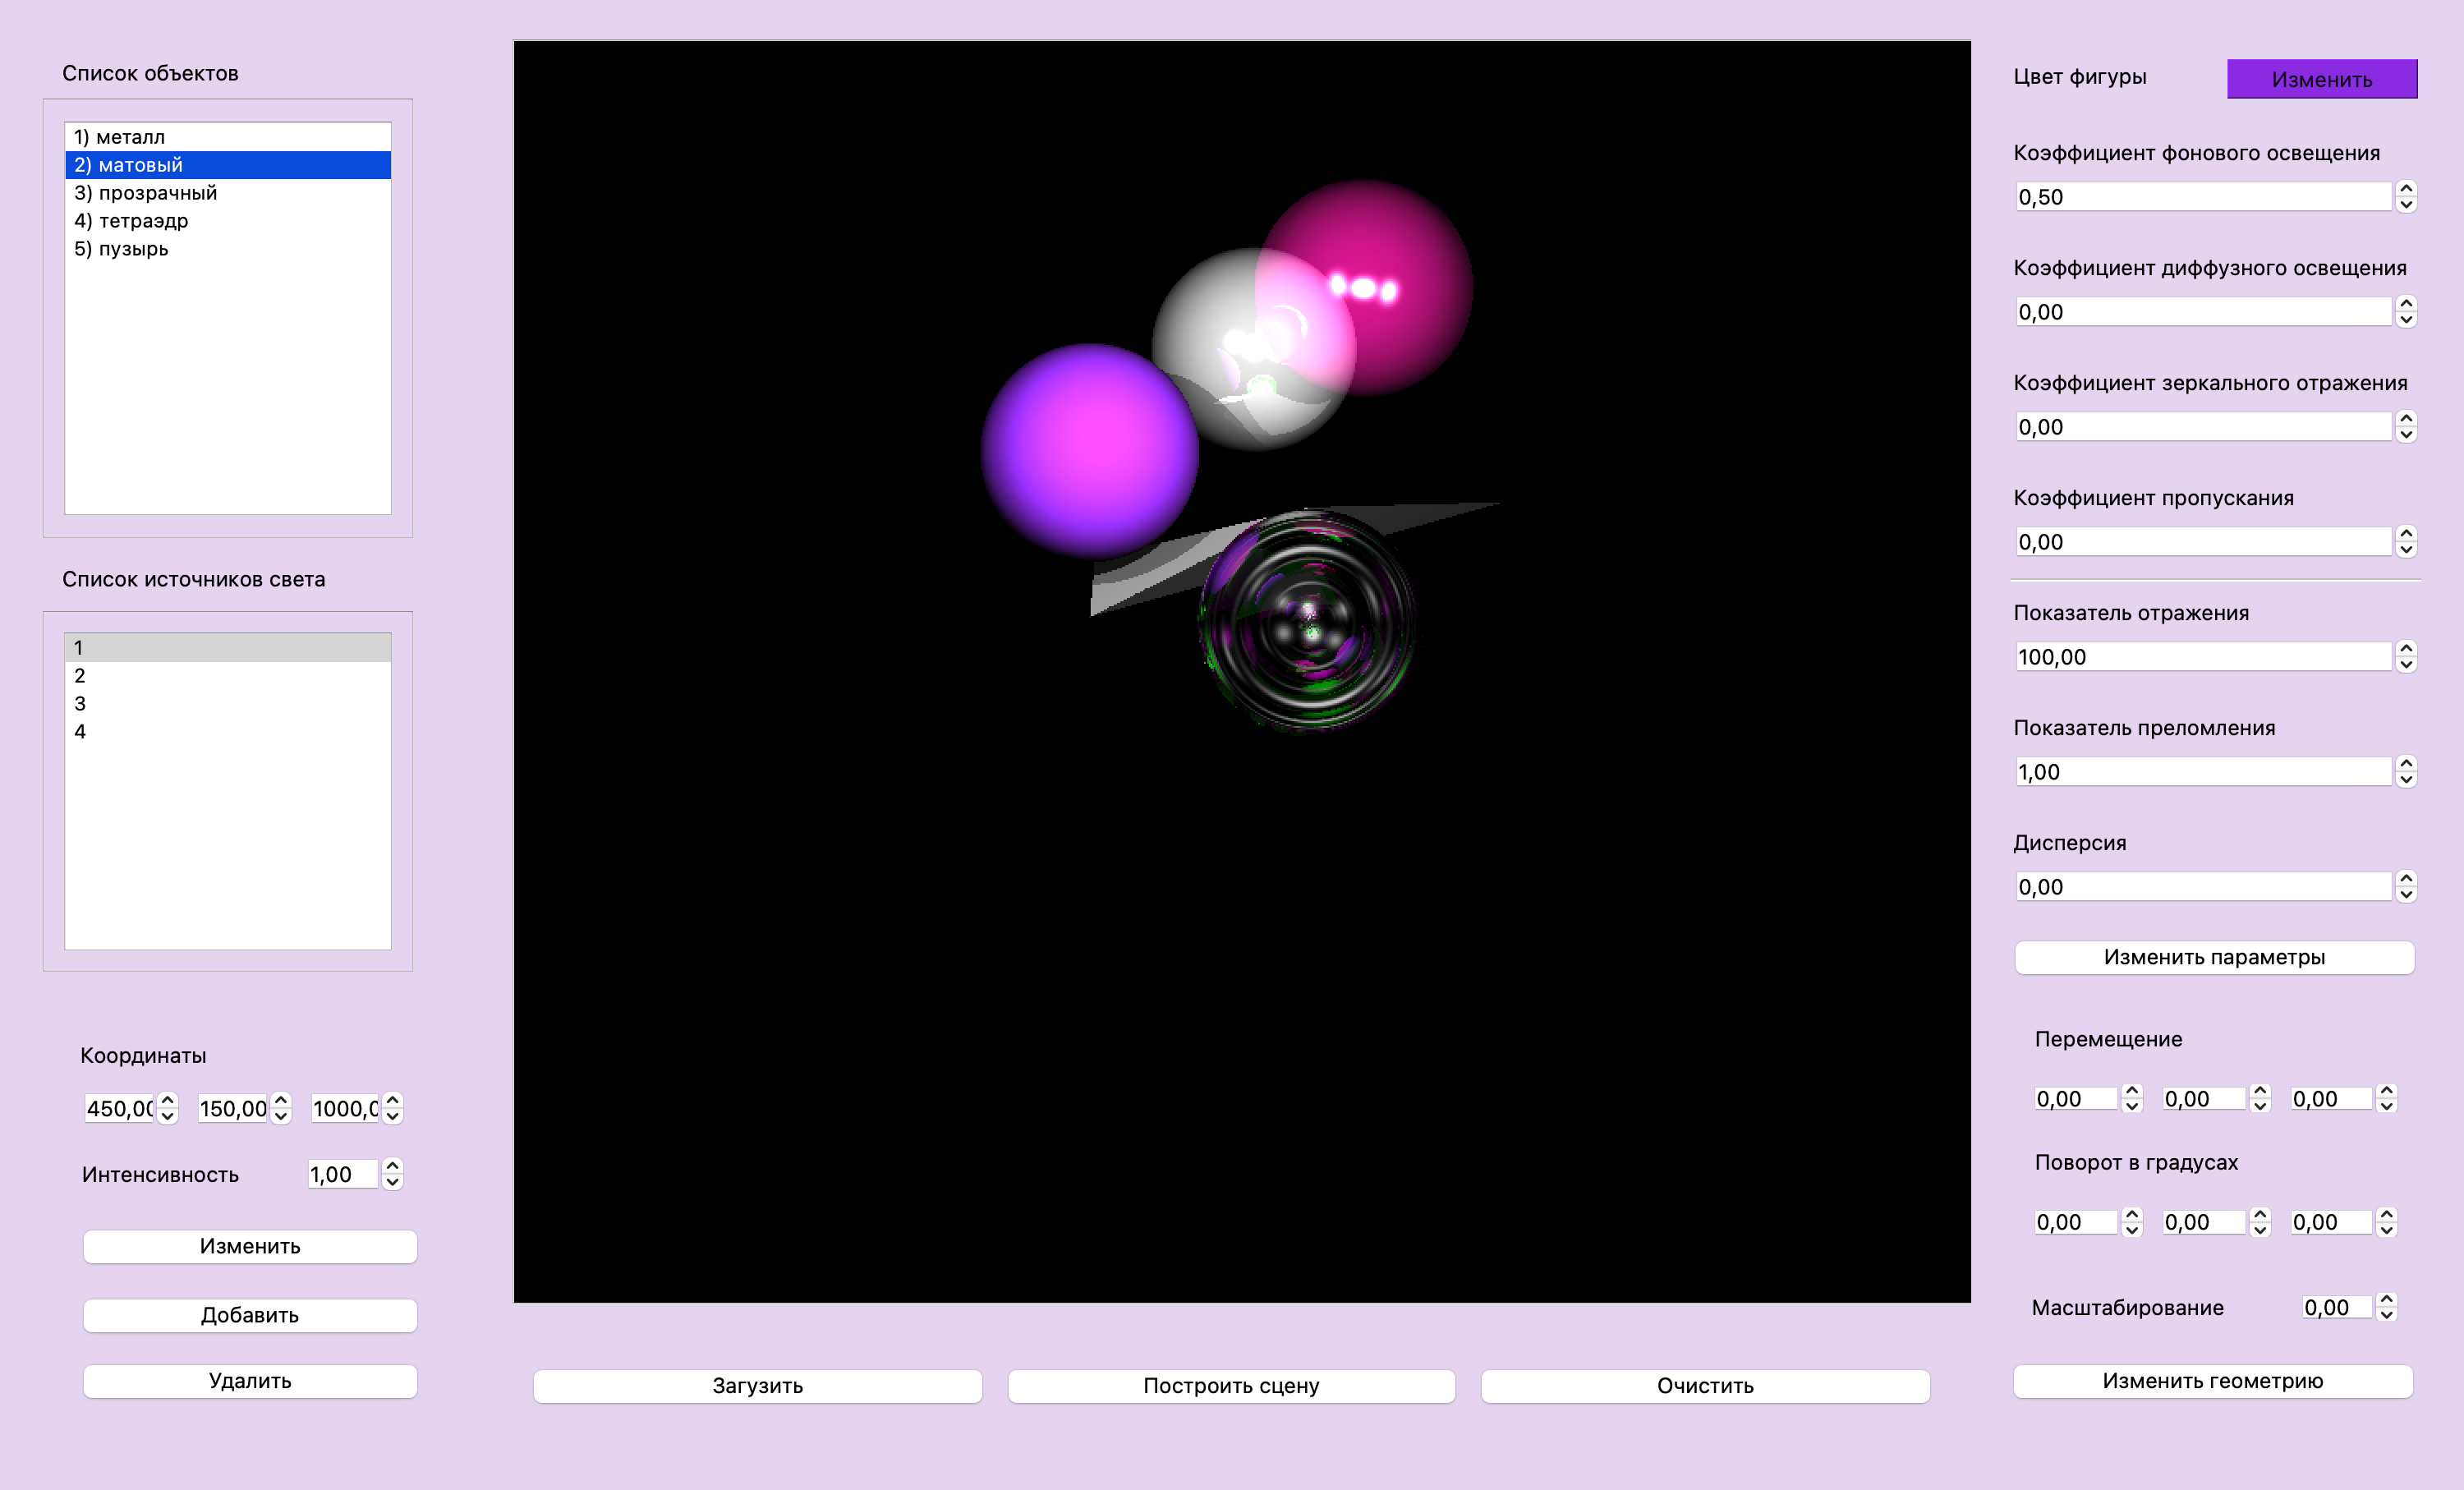
\includegraphics[width=\linewidth]{img/interface.png}
	\end{center}
	\captionsetup{justification=centering}
	\caption{Пример работы программы}
	\label{img:interface}
\end{figure}

С помощью реализованного интерфейса можно:

\begin{itemize}[label=---]
    \item загрузить объекты из файла, нажаd на кнопку <<Загрузить>> (названия объектов высветятся в окне <<Список объектов>>, а номера источников света в окне <<Список источников света>>);
    \item изменить положение источника и интенсивность, выделелив строку в окне <<Список источников света>>, записав новые значения и нажав на кнопку <<Изменить>>;
    \item добавить новый источник, введя его координаты и интенсивность и нажав на кнопку <<Добавить>>;
    \item удалить выделенный источник, нажав на кнопку <<Удалить>>.
    \item изменить оптические параметры объекта, выделив строку в окне <<Список объектов>>, указав новые значения и нажав на кнопку <<Изменить параметры>>;
    \item изменить расположение данного источника или увеличить его, указав коэффициенты преобразования и нажав на кнопку <<Изменить геометрию>>.
    \item очистить экран, нажав на кнопку <<Очистить>>.
\end{itemize}



% =====================================================
\section{Модульное тестирование}

Было проведено модульное тестирование с помощью фреймворка $Google Test$ \cite{gtest}.

В листинге \ref{lst:test} пример тестирования функции нахождения пересечения луча со сферой, код которой был представлен на листинге \ref{lst:tr}.

\begin{center}
\captionsetup{justification=raggedright,singlelinecheck=off}
\begin{lstlisting}[label=lst:test,caption=Тест для функции нахождения пересечения луча со сферой,basicstyle=\ttfamily\footnotesize]
TEST(SphereIntersectionTest, TwoIntersections) {
    Sphere sphere(QVector3D(0, 0, 0), 2.0);
    QVector3D start_point(0, 3, 0);
    QVector3D direction(0, -1, 0);
    double min_dist = 0.0;
    double max_dist = 10.0;

    auto intersectionInfo = sphere.getIntersectionInfo(start_point, direction, min_dist, max_dist);

    EXPECT_EQ(std::get<0>(intersectionInfo), QVector3D(0, 2, 0));
    EXPECT_EQ(std::get<2>(intersectionInfo), 1.0);
}
\end{lstlisting}
\end{center}

C помощью макроса \texttt{TEST} создаются тесты, а с помощью макроса \texttt{EXPECT\_EQ} проверяется совпадение результата с заранее вычесленным.

Были созданы наборы тестов для функций сцены, сферы и триангулированного объекта. Все тесты были пройдены успешно.


% =====================================================
\section{Функциональное тестирование}

Этапы проведения функционального тестирования изображены на рисунке \ref{img:func_test}.

\begin{figure}[H]
	\begin{center}
		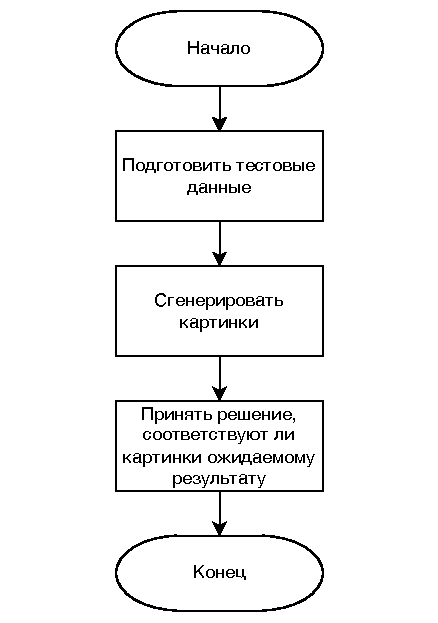
\includegraphics[width=0.5\linewidth]{img/func_test.pdf}
	\end{center}
	\captionsetup{justification=centering}
	\caption{Схема алгоритма проведения функционального тестирования}
	\label{img:func_test}
\end{figure}

В качестве функционального тестирования били построены все типы объектов, которые есть в программе: сфера, мыльный пузырь, триангулированный объект и источник света.

На рисунке \ref{img:func_1} продемонстрировано отражение фиолетовой сферы, перекрытой розовой сферой, в тетраэдре.

На рисунке \ref{img:func_2} продемонстрировано рекурсивное отражение фиолетовой сферы и тетраэдра и прозрачная розовая сфера, за которой видно тетраэдр.

На рисунке \ref{img:func_3} продемонстрирован мыльный пузырь и сферы, имеющие следующие оптические характеристики:
\begin{itemize}
	\item розовая сфера -- стеклянная (присутствуют отражение и преломление);
    \item серая сфера -- металлическая (присутствует только отражение);
    \item фиолетовая сфера -- матовая (отсутствуют отражение и преломление).
\end{itemize}

\begin{figure}[h]
	\begin{center}
		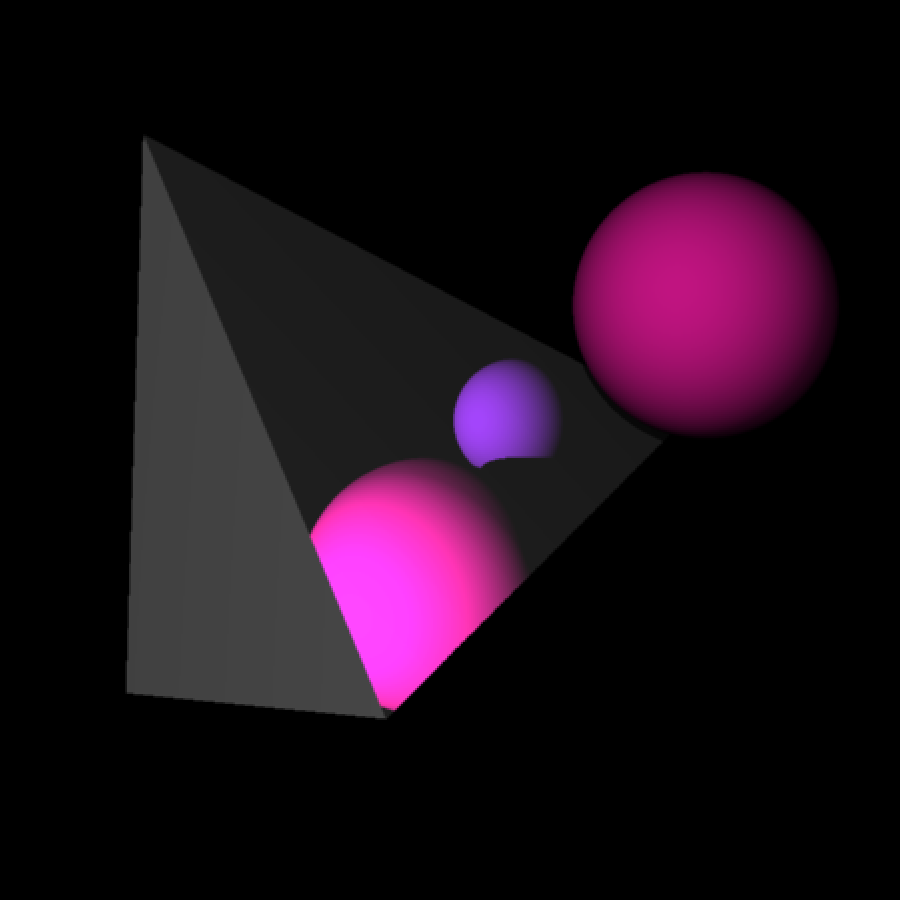
\includegraphics[width=0.9\linewidth]{img/func_1.png}
	\end{center}
	\captionsetup{justification=centering}
	\caption{Пример отражения перекрытого объекта}
	\label{img:func_1}
\end{figure}

\begin{figure}[h]
	\begin{center}
		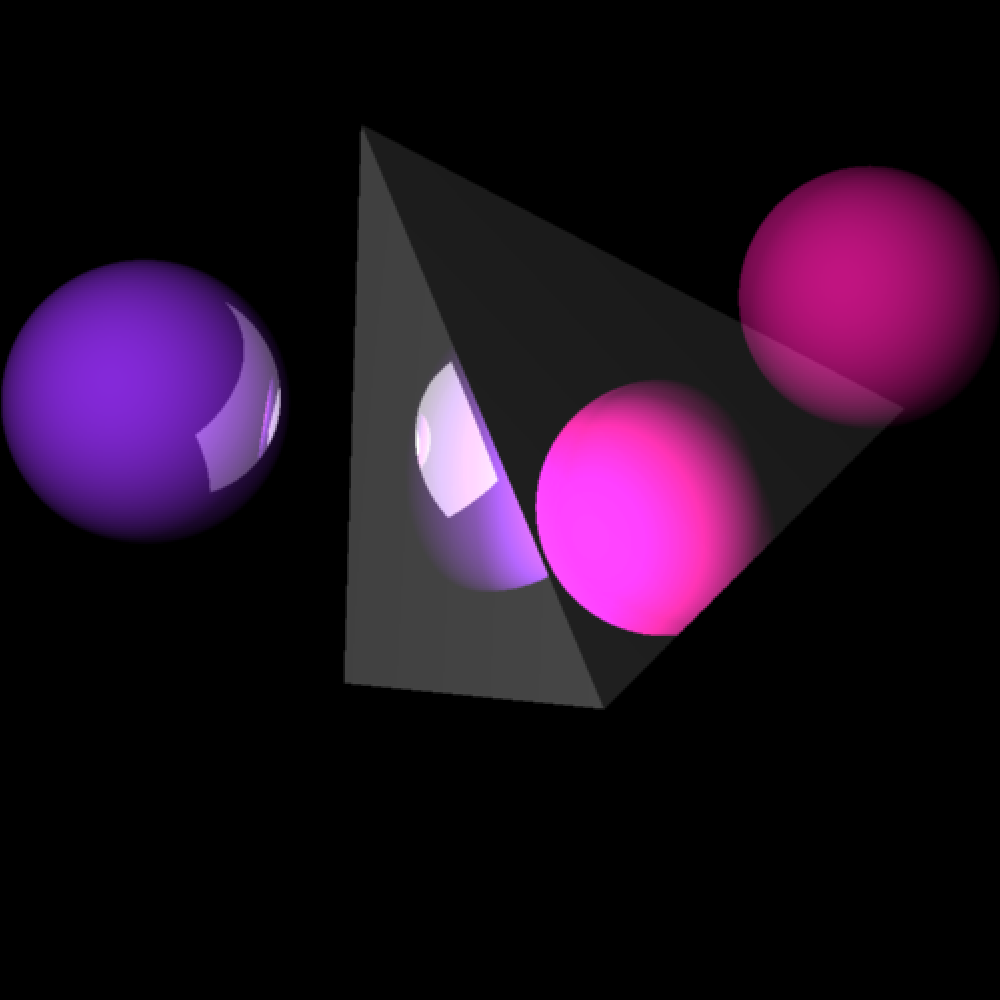
\includegraphics[width=0.9\linewidth]{img/func_2.png}
	\end{center}
	\captionsetup{justification=centering}
	\caption{Пример рекурсивного отражения и прозрачности}
	\label{img:func_2}
\end{figure}

\begin{figure}[h]
	\begin{center}
		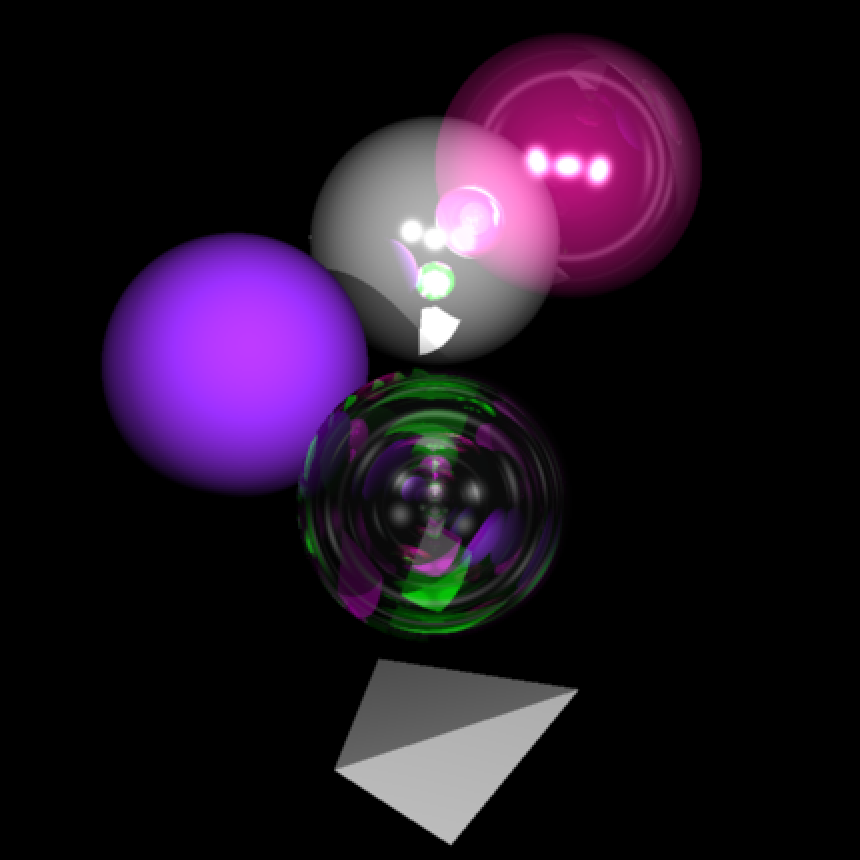
\includegraphics[width=0.9\linewidth]{img/func_3.png}
	\end{center}
	\captionsetup{justification=centering}
	\caption{Пример мыльного пузыря и сфер из различных материалов}
	\label{img:func_3}
\end{figure}

\clearpage


% =====================================================
\section{Интерфейс управления из командной строки}

Для автоматизации некоторых процессов в программе реализовано управление из командной строки:

\begin{itemize}
	\item ключ <<-image>>, после которого идет название текстового файла, в котором описаны объекты, а далее название изображения, получаемого при работе программы;
	\item ключ <<-film>>, после которого идет название текстового файла, в котором описаны объекты, далее название фильма, получаемого при работе программы и в конце название текстового файла, в котором хранятся команды для модификации сцены;
	\item ключ <<-research>>, после которого идет название текстового файла, в котором описаны объекты, далее название изображения, получаемого при работе программы и в конце значение глубины трассировки (целое неотрицательное число).
\end{itemize}

%=====================================================
\section{Выводы из технологической части}

В технологической части были выбраны средства реализации и реализовано спроектированное программное обеспечение. Кроме того, были продемонстрированы примеры работы программы и проведено тестирование.
